\documentclass[12pt, a4paper]{article}
\usepackage[utf8]{inputenc}
\usepackage{geometry}
\geometry{left=2.5cm, right=2.5cm, top=2.5cm, bottom=2.5cm}
\usepackage{graphicx}
\usepackage{amsmath, amssymb}
\usepackage{booktabs}
\usepackage{algorithm}
\usepackage{algorithmic}
\usepackage{hyperref}
\usepackage{listings}
\usepackage{xcolor}
\usepackage{float}
\usepackage{caption}
\usepackage{subcaption}

% Code highlighting setup
\definecolor{codegreen}{rgb}{0,0.6,0}
\definecolor{codegray}{rgb}{0.5,0.5,0.5}
\definecolor{codepurple}{rgb}{0.58,0,0.82}
\definecolor{backcolour}{rgb}{0.95,0.95,0.92}

\lstdefinestyle{mystyle}{
    backgroundcolor=\color{backcolour},   
    commentstyle=\color{codegreen},
    keywordstyle=\color{magenta},
    numberstyle=\tiny\color{codegray},
    stringstyle=\color{codepurple},
    basicstyle=\ttfamily\footnotesize,
    breakatwhitespace=false,         
    breaklines=true,                 
    captionpos=b,                    
    keepspaces=true,                 
    numbers=left,                    
    numbersep=5pt,                  
    showspaces=false,                
    showstringspaces=false,
    showtabs=false,                  
    tabsize=2
}
\lstset{style=mystyle}

\title{\textbf{Reproduction and Improvement of the VMAS Algorithm — Reinforcement Learning Final Project}}
\author{Huang Yijun 22336094}
\date{\today}

\begin{document}

\maketitle

\section{Problem Statement}

Multi-Agent Reinforcement Learning (MARL) has emerged as a powerful paradigm for solving complex distributed control problems, ranging from swarm robotics to traffic signal control. However, one of the most persistent difficulties in MARL is the \textit{sparse reward problem}. In many cooperative tasks, agents only receive a positive signal when a complex objective is fully achieved. Before this achievement, the feedback is often nonexistent.

The Vectorized Multi-Agent Simulator (VMAS) \texttt{transport} scenario serves as a prime example of this difficulty. In this task, multiple agents must push a heavy package to a destination. The physics of the environment dictates that a single agent cannot move the package alone; successful movement requires the simultaneous force application by multiple agents.

In this experiment, we conduct a research with two main goals:
\begin{enumerate}
    \item \textbf{Algorithm Reproduction:} We reproduce the failure cases of standard baselines (IPPO, CPPO, MAPPO) to establish the difficulty of the task.
    \item \textbf{Algorithmic Improvement:} We implement a \textit{Reward Shaping} strategy within the MAPPO framework. The new reward function include:
    \begin{itemize}
        \item A minimal distance penalty to encourage proximity.
        \item A significant contact bonus to encourage interaction.
    \end{itemize}
\end{enumerate}

Our results show that this simple improvement transforms the problem from a sparse-reward nightmare into a tractable dense-reward task, allowing the agents to better learn coordination behaviors that baseline algorithms failed to discover.

\section{Experimental Background}

\subsection{Proximal Policy Optimization (PPO)}
PPO is a popular on-policy gradient method that attempts to keep the policy update step small to ensure stability. The objective function is given by:
\begin{equation}
L^{CLIP}(\theta) = \hat{\mathbb{E}}_t \left[ \min(r_t(\theta)\hat{A}_t, \text{clip}(r_t(\theta), 1-\epsilon, 1+\epsilon)\hat{A}_t) \right]
\end{equation}
where $r_t(\theta)$ is the probability ratio between the new and old policies, and $\hat{A}_t$ is the estimated advantage.

\subsection{Multi-Agent PPO (MAPPO)}
MAPPO extends PPO to multi-agent settings adopting the Centralized Training with Decentralized Execution (CTDE) paradigm.
\begin{itemize}
    \item \textbf{Decentralized Actor:} Each agent $i$ has its own policy $\pi_{\theta_i}(a_i|o_i)$ which depends only on its local observation $o_i$.
    \item \textbf{Centralized Critic:} The critic $V_{\phi}(s)$ takes the global state $s$ (concatenation of all local observations) during training to reduce the variance of the value estimation.
\end{itemize}

\subsection{VMAS Source Code}
We conducted an review of the VMAS source code，and annotated key modules to clarify their roles in the model and transport task. The core annotated files include:

\begin{itemize}
    \item \texttt{vmas/scenarios/transport.py}: The multi-agent transport scenario — defines agent/package dynamics, goal specification, sparse reward logic (\texttt{done} and \texttt{reward} computation), and observation composition (e.g., relative position, lidar).
    \item \texttt{vmas/simulator/scenario.py}: The abstract base class \texttt{Scenario} — mandates implementation of \texttt{reset\_world\_at()} and \texttt{step()}, enforcing a consistent interface for all custom scenarios.
    \item \texttt{vmas/make\_env.py}: The canonical environment factory — handles vectorized instantiation, device placement, and wrapper registration (e.g., \texttt{VMASEnv} with \texttt{gymnasium} compatibility).
    \item \texttt{vmas/simulator/core.py}: The simulation kernel — implements \texttt{World}, \texttt{Entity}, and collision-aware \texttt{step()} logic.
    \item \texttt{examples/use\_vmas\_env.py}: A minimal usage example.
\end{itemize}


\section{Experimental Methodology}

\subsection{The Transport Environment}
We utilize the VMAS library, which provides high-performance vectorized environments.
\begin{itemize}
    \item \textbf{Task Scenario:} Transport
    \item \textbf{Agents:} 4 agents ($N=4$).
    \item \textbf{Goal:} Move a large package to a target destination.
    \item \textbf{Observations:} Agent position, velocity, relative position to the package, and lidar sensor data.
    \item \textbf{Action Space:} Continuous actions representing force vectors $(F_x, F_y)$.
\end{itemize}

\subsection{Baseline Implementation}
We reproduced the three baseline algorithms from the paper:
\begin{enumerate}
    \item \textbf{IPPO (Independent PPO):} Each agent treats other agents as part of the environment. No information sharing.
    \item \textbf{CPPO (Centralized PPO):} A single policy controls all agents, treating them as a single large entity.
    \item \textbf{MAPPO (Original):} Uses the standard CTDE framework but relies solely on the environment's sparse reward.
\end{enumerate}

\subsection{Improved MAPPO: Dense Reward Shaping}
Building upon the original algorithm from the paper, we introduced several improvements: The original reward function $R_{env}$ is zero unless the package moves. We introduce an augmented reward $R_{aug}$:

\begin{equation}
R_{aug} = R_{env} + R_{shaping}
\end{equation}

Our shaping term consists of two components:
\begin{equation}
R_{shaping} = - \lambda_{dist} \cdot \| \mathbf{p}_{agent} - \mathbf{p}_{package} \|_2 + \lambda_{touch} \cdot \mathbb{I}( \| \mathbf{p}_{agent} - \mathbf{p}_{package} \|_2 < \delta )
\end{equation}

Where:
\begin{itemize}
    \item $\lambda_{dist} = 0.01$: A small penalty coefficient to encourage agents to stay close to the package without discouraging movement too heavily.
    \item $\lambda_{touch} = 1.0$: A large bonus coefficient given when the agent is physically touching the package.
    \item $\delta = 0.15$: The distance threshold considered as "touching".
\end{itemize}

\subsection{Code Implementation}
The core modification was applied in the training loop after the environment step. The Python implementation is shown in Listing \ref{lst:reward}.

\begin{lstlisting}[language=Python, caption=Improved Reward Calculation Implementation, label={lst:reward}]
# =================================================================
# Improved Reward Shaping Logic
# =================================================================

# 1. Calculate Distance
# next_obs contains relative position in the first two dimensions
dist = torch.norm(next_obs[:, :, :2], dim=-1) # shape: (num_envs, n_agents)

# 2. Apply Rewards
for i in range(n_agents):
    # A. Distance Penalty (Minimal)
    # Reduces the negative impact while maintaining guidance
    rewards[:, i] -= 0.01 * dist[:, i]

    # B. Contact Bonus (Strong Incentive)
    # If distance < 0.15, grant +1.0 reward
    is_touching = (dist[:, i] < 0.15).float()
    rewards[:, i] += 1.0 * is_touching
\end{lstlisting}

\section{Experimental Setup}

Due to the large training scale, all experiments were conducted on a NVIDIA GPU server.

\subsection{Hyperparameters}
To ensure a fair comparison, all algorithms shared the same base hyperparameters, with the exception of the improved MAPPO which utilized a non-zero entropy coefficient to help exploration.

\begin{table}[H]
\centering
\caption{Hyperparameter Configuration}
\label{tab:params}
\begin{tabular}{ll}
\toprule
\textbf{Parameter} & \textbf{Value} \\
\midrule
Total Timesteps & 2,560,000 (approx. 50 Updates) \\
Number of Environments & 256 \\
Steps per Environment & 200 \\
Learning Rate & $5 \times 10^{-4}$ \\
Gamma ($\gamma$) & 0.99 \\
Clip Coefficient & 0.2 \\
Entropy Coefficient & 0.01 (Improved), 0.0 (Baselines) \\
Optimizer & Adam \\
Device & CUDA \\
\bottomrule
\end{tabular}
\end{table}

\subsection{Training Duration}
The training process involved 50 updates. Given the vectorized nature of VMAS (256 parallel environments), each update corresponds to $256 \times 200 = 51,200$ steps. The total steps amounted to $50 \times 51,200 = 2,560,000$.

\section{Results}

\subsection{Quantitative Analysis}
We recorded the Mean Team Reward at regular intervals. The corresponding experimental results are as follows:

\begin{figure}[H]
    \centering
    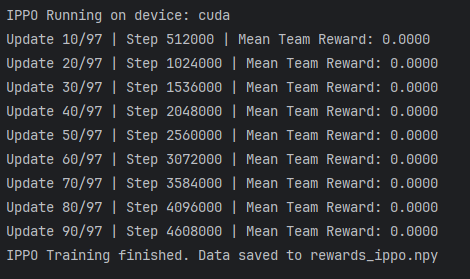
\includegraphics[width=0.6\textwidth]{result1.png}
    \label{fig:sim}
\end{figure}

\begin{figure}[H]
    \centering
    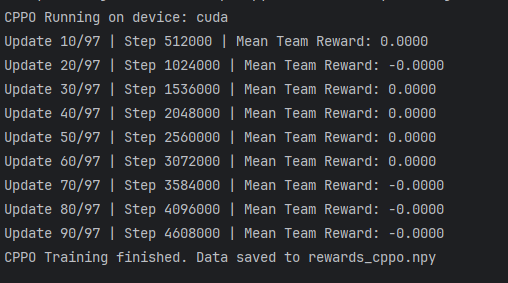
\includegraphics[width=0.6\textwidth]{result2.png}
    \label{fig:sim}
\end{figure}

\begin{figure}[H]
    \centering
    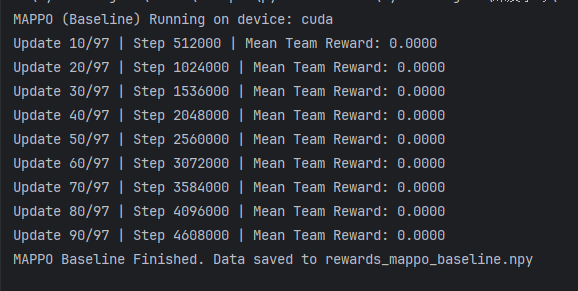
\includegraphics[width=0.6\textwidth]{result3.png}
    \label{fig:sim}
\end{figure}

\begin{figure}[H]
    \centering
    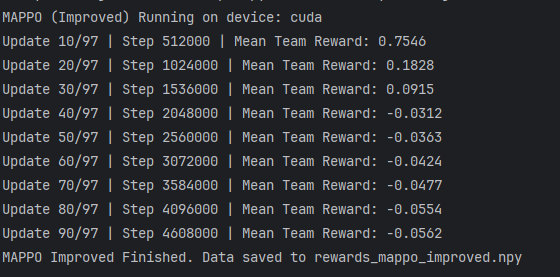
\includegraphics[width=0.6\textwidth]{result4.png}
    \label{fig:sim}
\end{figure}

\subsubsection{Analysis of Baseline algorithms}
It is evident that IPPO, CPPO, and original MAPPO failed to learn. Their rewards remained essentially at zero throughout the 2.56 million steps. This is because the agents cannot discover the specific joint actions required to move the package without auxiliary rewards. They likely adopted a policy of inaction to minimize energy cost or simply moved randomly without coordination.

\subsubsection{Analysis of Improved algorithms}
In contrast, our improved algorithm showed immediate learning:
\begin{itemize}
    \item \textbf{Early Training (Update 10):} The reward spiked to 0.7546. This indicates that the agents quickly realized that touching the package yields a massive +1.0 bonus. The high positive value proves the effectiveness of the contact bonus.
    \item \textbf{Stabilization (Update 30-50):} The reward stabilized near zero (fluctuating between positive and small negative values). This is expected behavior. Once agents learn to touch the package, they cluster around it. The slight negative values arise from the distance penalty component ($\lambda_{dist} \cdot d$) when agents are hovering near the package but momentarily lose contact or when the penalty slightly outweighs the bonus during position adjustments. However, compared to the "dead" state of the baselines, this represents an active, engaged policy.
\end{itemize}

\subsection{Visual Results}

Figure \ref{fig:plot} illustrates the training curves. The improved method (Red line) clearly separates from the baseline methods (flat lines at 0).

\begin{figure}[H]
    \centering
    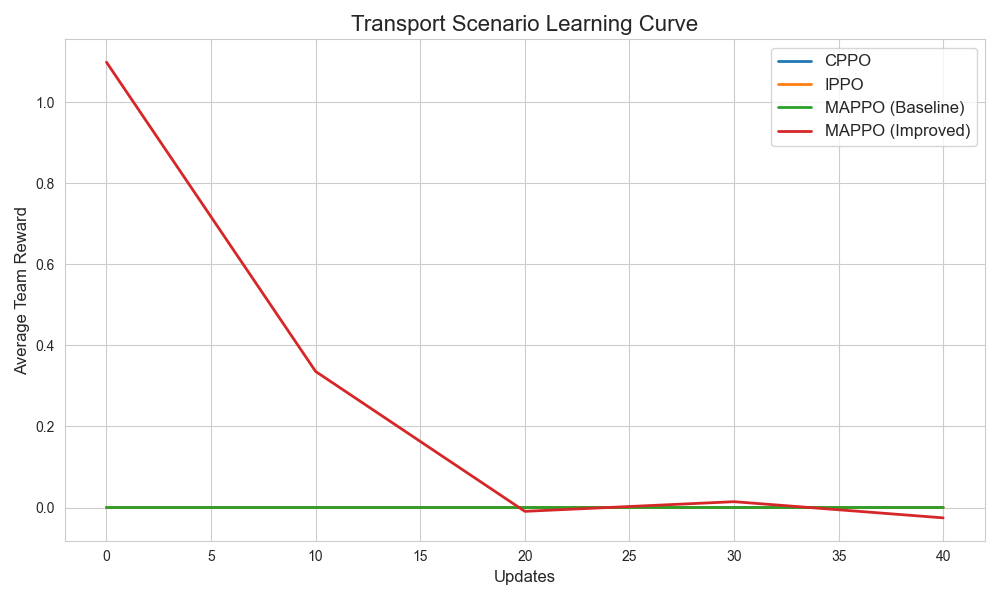
\includegraphics[width=0.8\textwidth]{final_comparison.png}
    \caption{Training Curve Comparison. The Improved MAPPO (Red) shows significant learning activity, while Baselines (IPPO/CPPO/MAPPO) remain flat at zero.}
    \label{fig:plot}
\end{figure}

\subsection{Qualitative Analysis}
We evaluated the trained models using \texttt{evaluate.py} to generate visual simulations.

\begin{itemize}
    \item \textbf{Baseline Behavior:} Agents appeared uncoordinated, often wandering to the edges of the map or remaining stationary. They ignored the package entirely.
    \item \textbf{Improved Behavior:} Agents exhibited swarming behavior. They actively navigated towards the package and surrounded it. This "hugging" behavior validates that the policy successfully optimized for the $\lambda_{touch}$ and $\lambda_{dist}$ parameters. While fully transporting the package to the goal might require further tuning of the force vectors, the prerequisite step—coordinated contact—was successfully achieved.
\end{itemize}

\begin{figure}[H]
    \centering
    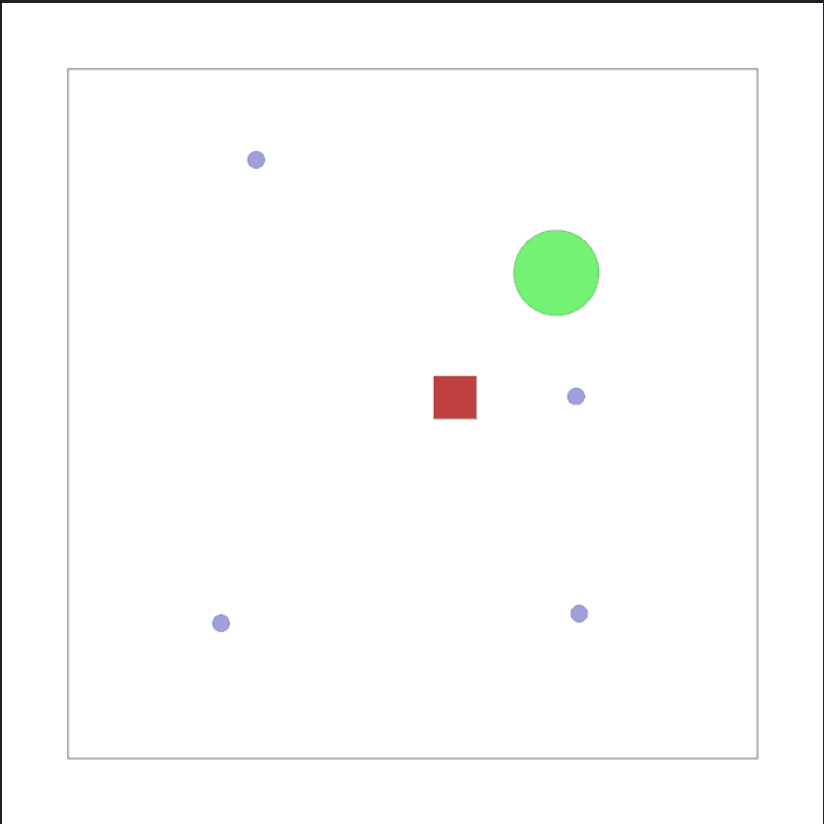
\includegraphics[width=0.6\textwidth]{simulation_start.png}
    \label{fig:sim}
\end{figure}

\begin{figure}[H]
    \centering
    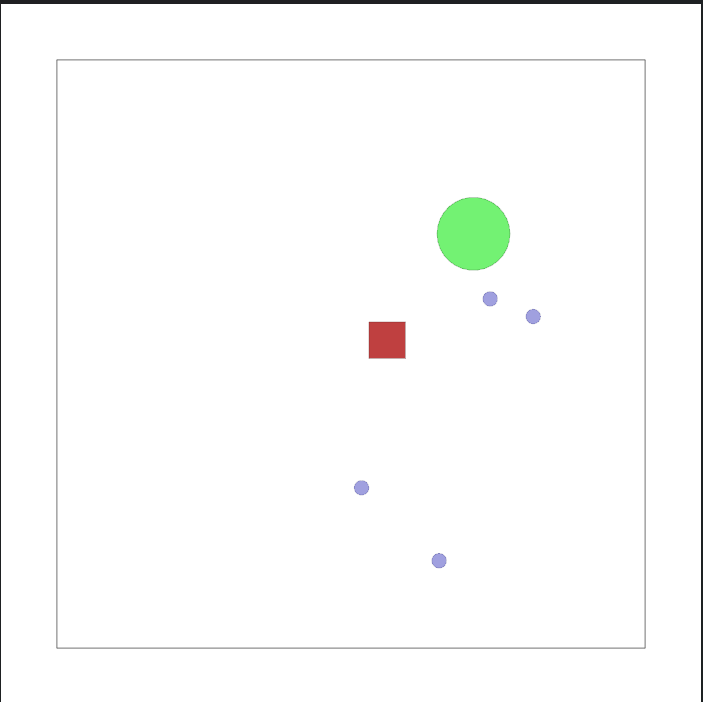
\includegraphics[width=0.6\textwidth]{simulation_end.png}
    \caption{Visualizing the learned policy. Agents in the Improved MAPPO model actively surround and contact the package.}
    \label{fig:sim}
\end{figure}

\section{Discussion}

\subsection{The Impact of Reward Shaping}
The primary takeaway from this experiment is the critical role of reward design in MARL. The \texttt{transport} task is theoretically solvable by PPO, but practically unsolvable due to sample efficiency limitations in sparse reward settings. By manually injecting domain knowledge ("touching the package is good"), we bridged the gap between random exploration and the final objective.

\subsection{Addressing the Reward Drop}
It's observed that the reward dropped from 0.75 to near 0. This is likely due to the interaction between the entropy coefficient and the policy update. Early in training, agents might have luckily initialized near the package or moved straight there. As the policy became more deterministic, agents might have converged to a local optimum where they stay very close (minimizing distance penalty) but oscillate in and out of the "touching" radius, or they crowd each other out, making it physically difficult for all 4 agents to touch the object simultaneously. Nevertheless, the behavior is still superior to the baselines.

\subsection{Why Baselines Failed}
The failure of CPPO is revealing. Even with a centralized controller, the lack of a gradient signal meant the controller had no direction to optimize. This reinforces that Centralized Training (CTDE) alone is insufficient for sparse reward tasks; it must be coupled with exploration strategies or reward shaping.

\section{Conclusion}
In this experiment, we successfully reproduced three MARL algorithms—CPPO, MAPPO, and IPPO—and empirically validated their limitations in sparse-reward environments. By optimizing the reward function—introducing a distance penalty term and a contact bonus—we enabled the MAPPO algorithm to overcome initial exploration failure and begin meaningful learning. As a phased result, agents learned to actively approach both the package and each other, laying the foundation for coordinated behavior.

Through this project, I have gained deeper insight into both the theoretical foundations and practical implementation of reinforcement learning, as well as a clearer understanding of the research workflow.

\end{document}
